\documentclass{article}
\usepackage{geometry}
\usepackage{graphicx}
\usepackage{amsmath}
\usepackage{algorithm}
\usepackage{algpseudocode}
\usepackage{dsfont}
\usepackage{amssymb}
\usepackage{multicol}

\geometry{
a4paper,
right=10mm,
left=10mm,
top=10mm,
bottom=10mm,	
}

\begin{document}

\pagenumbering{gobble}

\begin{center}
\textbf{\Large HOMEWORK 2 : CS771} \\
\textit{\large Jayant Agrawal}         14282
\end{center}
\section{Problem 1}
\begin{figure}[h!]
\centering
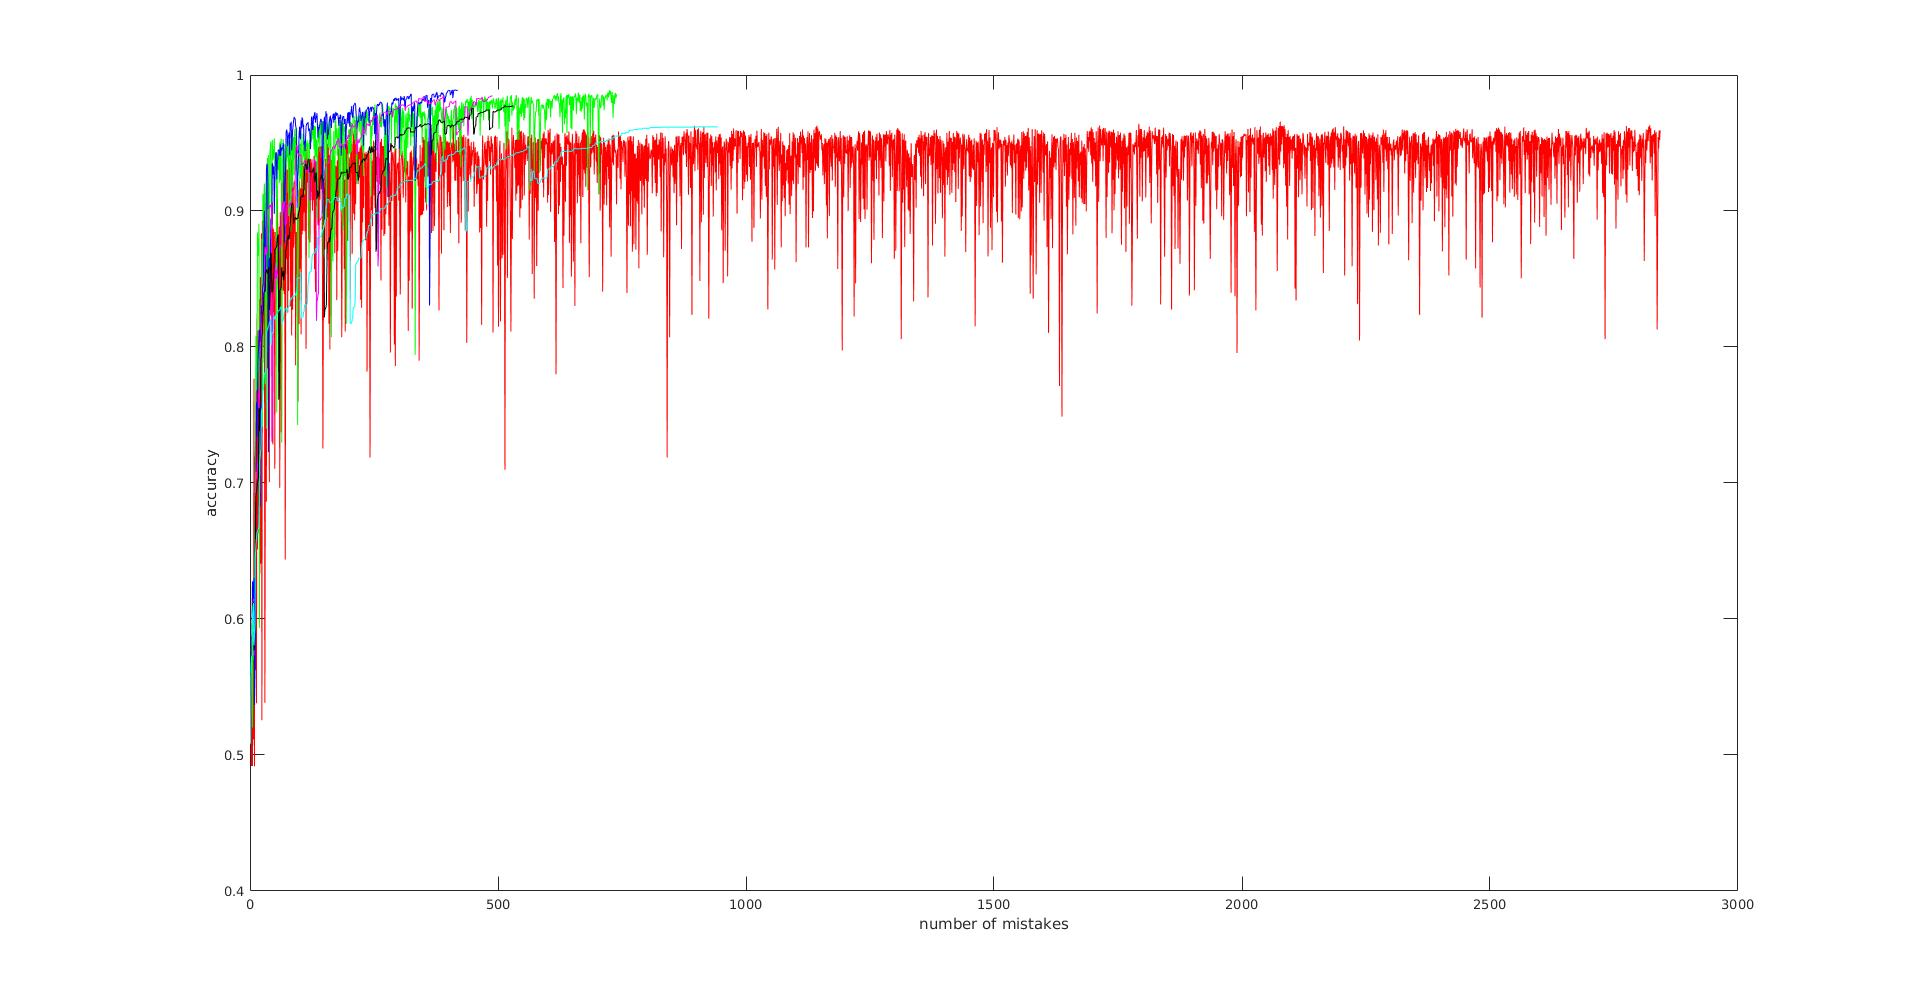
\includegraphics[width=0.8\columnwidth]{plot_acc.jpg}
\caption{Classification Accuracy: Simple(Red) and Averaged(Green)}
\label{acc}
\end{figure}

\section{Problem 2}
\subsection{Fig 1}
\begin{figure}[h!]
\begin{center}
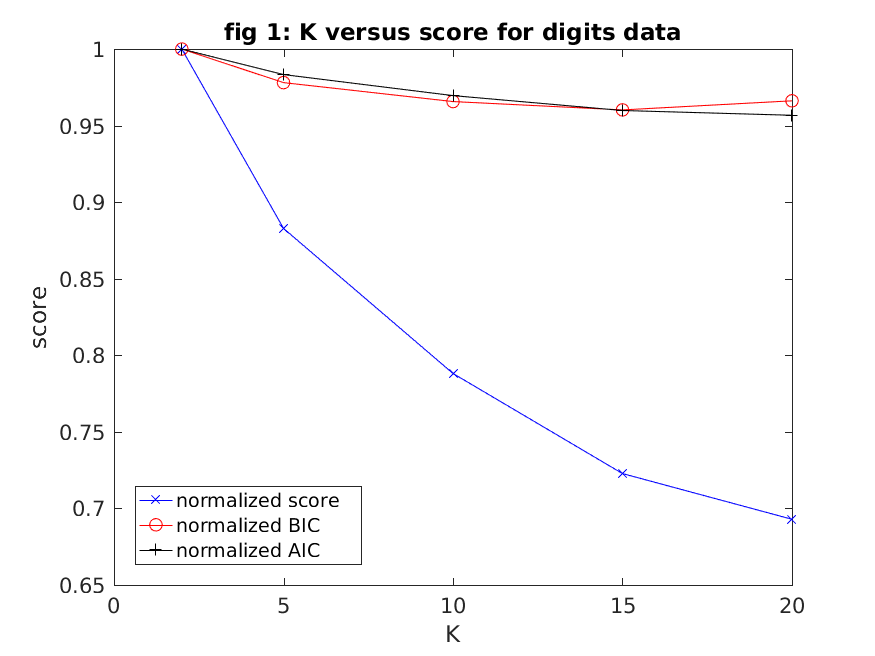
\includegraphics[width=0.5\columnwidth]{RunResults2/1.png}
\label{1}
\end{center}
\end{figure}
\newpage
\subsection{Fig 2}
\begin{figure}[h!]
\begin{center}
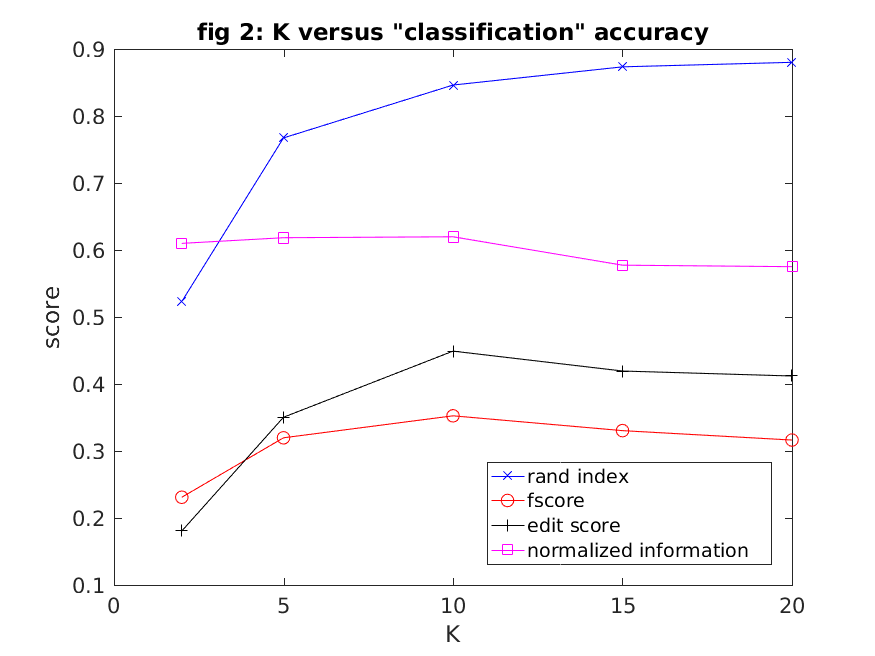
\includegraphics[width=.5\columnwidth]{RunResults2/2.png}
\label{2}
\end{center}
\end{figure}

\subsection{Fig 3-5}
%\begin{left}
\begin{figure}[h!]
\begin{multicols}{3}
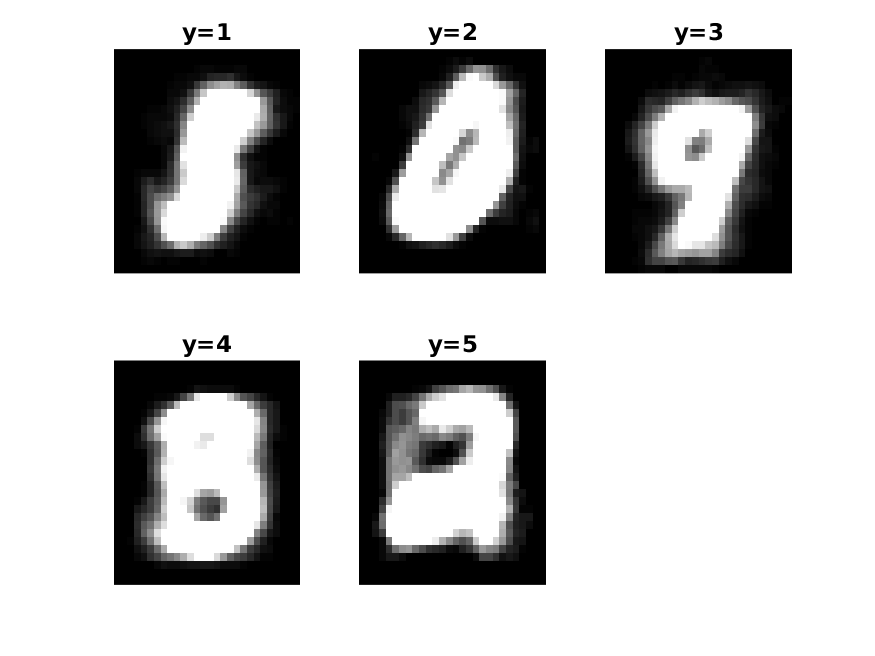
\includegraphics[width=1\columnwidth]{RunResults2/3.png}
\label{3}
%\caption{Fig 3}

%\end{left}
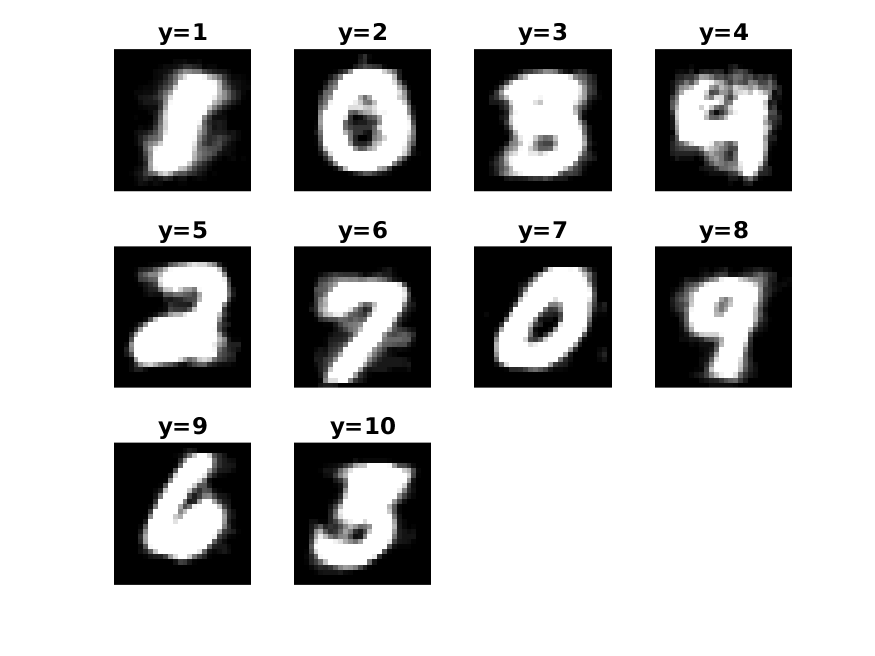
\includegraphics[width=1\columnwidth]{RunResults2/4.png}
\label{4}
%\caption{Fig 4}

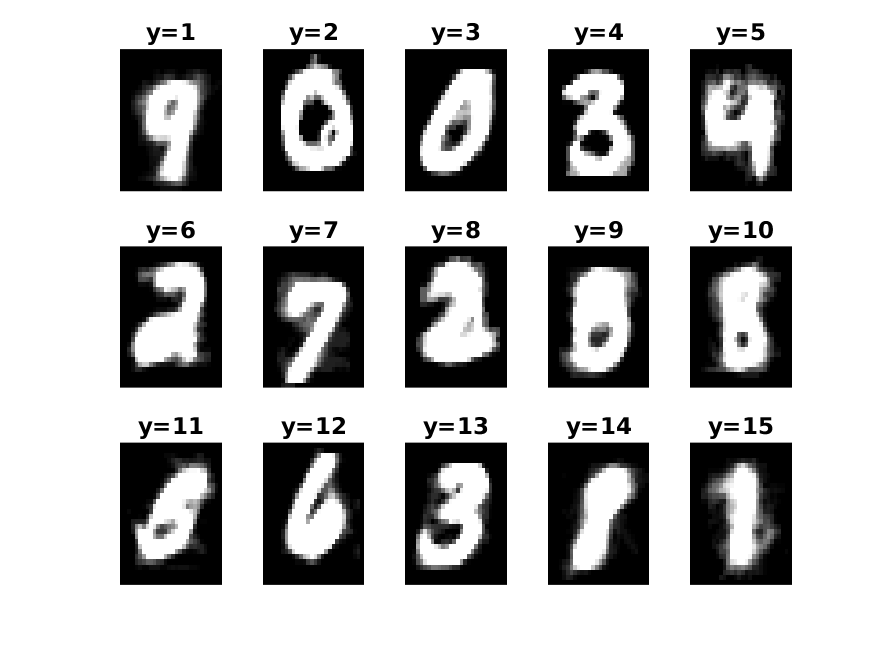
\includegraphics[width=1\columnwidth]{RunResults2/5.png}
\label{5}
%\caption{Fig 5}
\end{multicols}
\end{figure}

\subsection{Fig 6}
\begin{figure}[h!]
\begin{center}
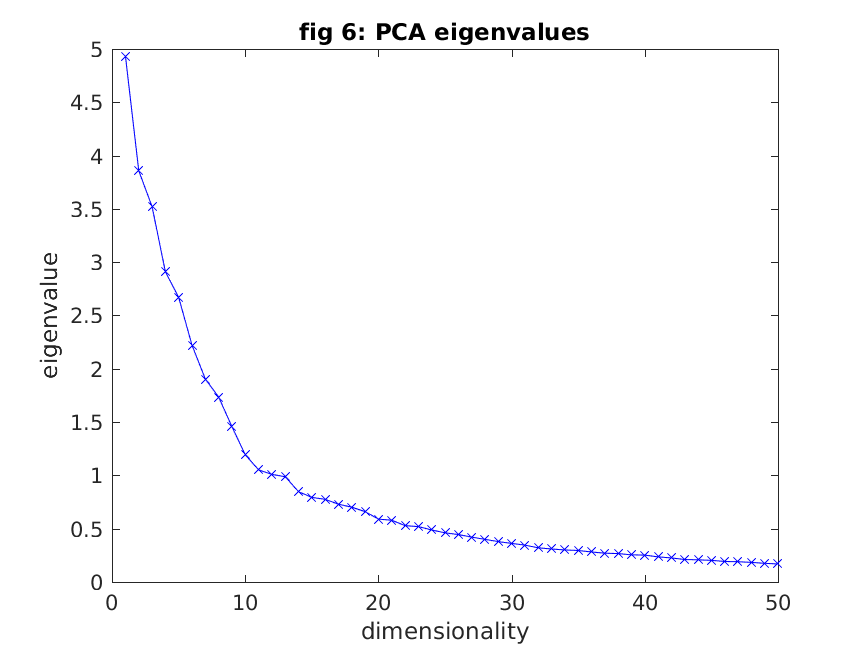
\includegraphics[width=0.5\columnwidth]{RunResults2/6.png}
\label{6}
\end{center}
\end{figure}
\newpage
\subsection{ Fig 7}
\begin{figure}[h!]
\begin{center}
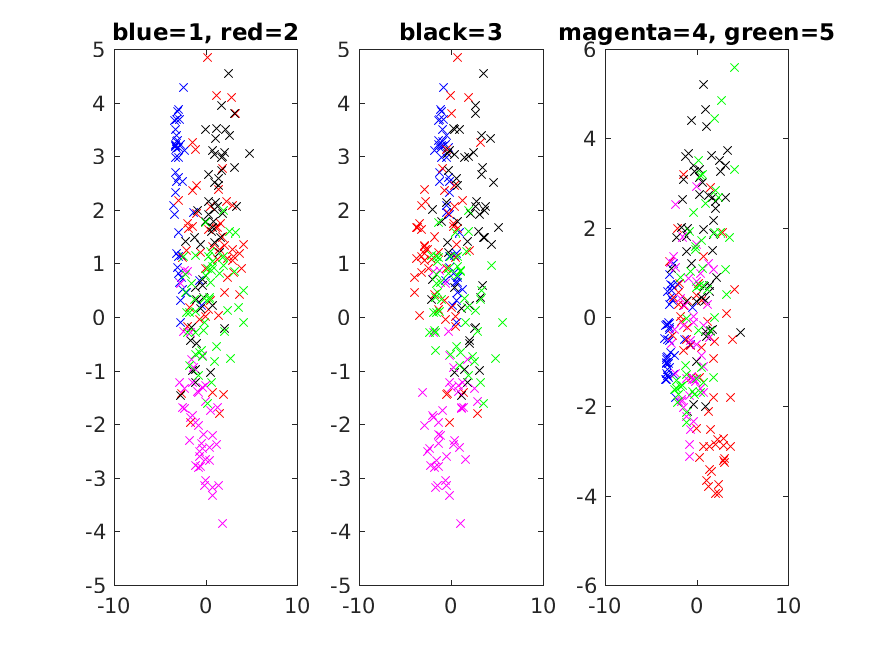
\includegraphics[width=0.5\columnwidth]{RunResults2/7.png}
\label{7}
\end{center}
\end{figure}

\subsection{Fig 8-12}
\begin{figure}[h!]
\begin{multicols}{3}
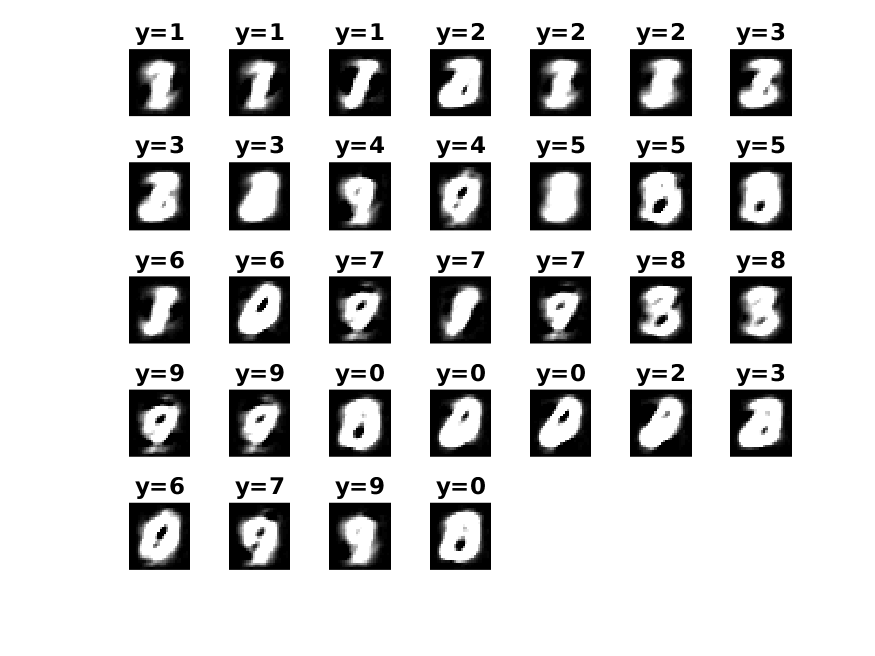
\includegraphics[width=1\columnwidth]{RunResults2/8.png}
\label{8}

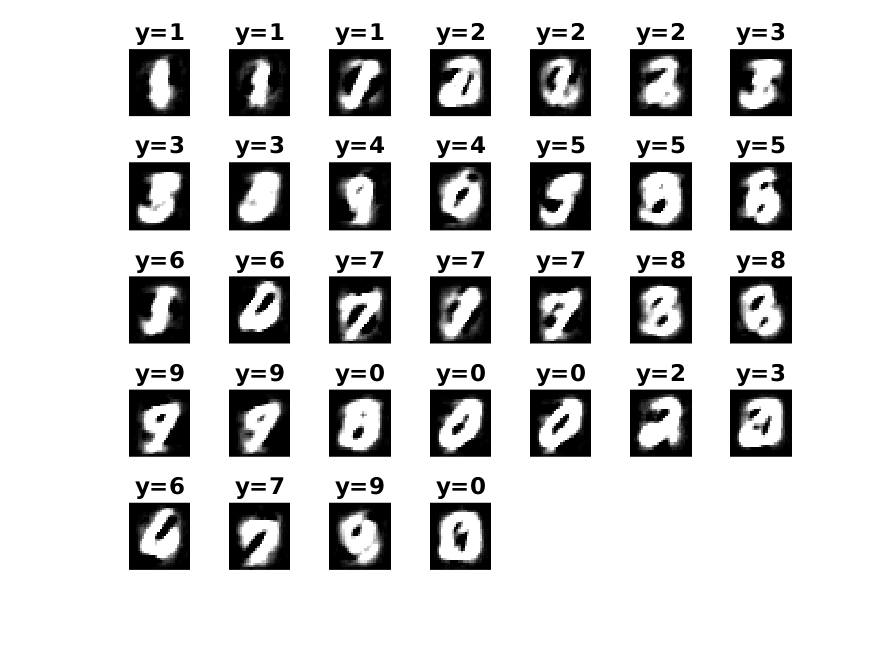
\includegraphics[width=1\columnwidth]{RunResults2/9.png}
\label{9}

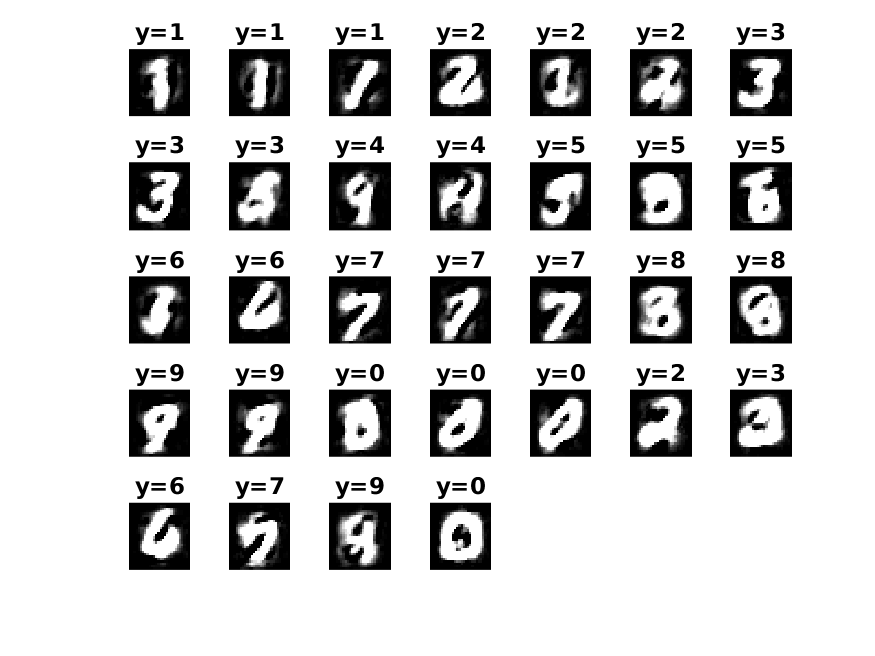
\includegraphics[width=1\columnwidth]{RunResults2/10.png}
\label{10}
\end{multicols}
\centering
\begin{multicols}{2}
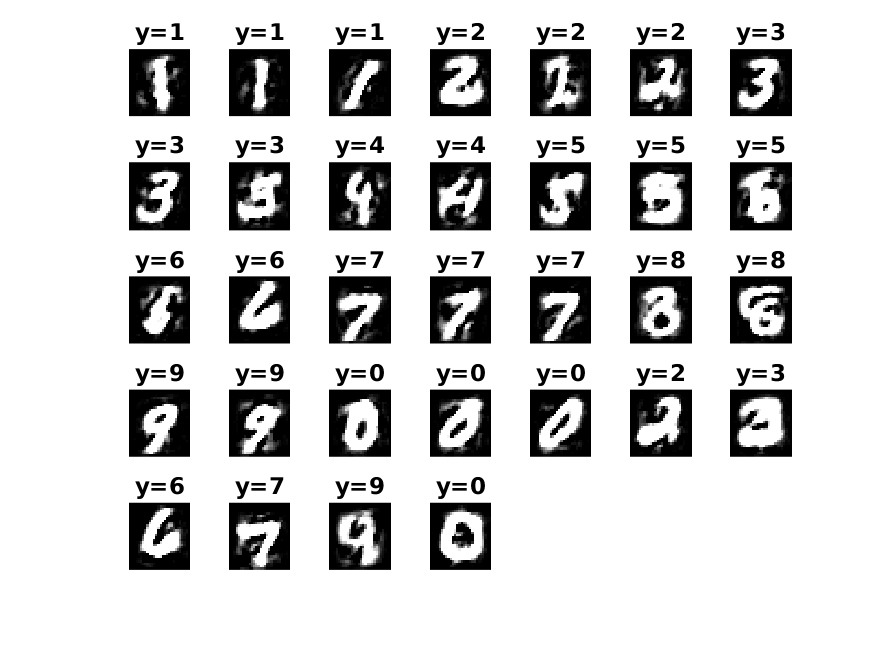
\includegraphics[width=0.65\columnwidth]{RunResults2/11.png}
\label{11}

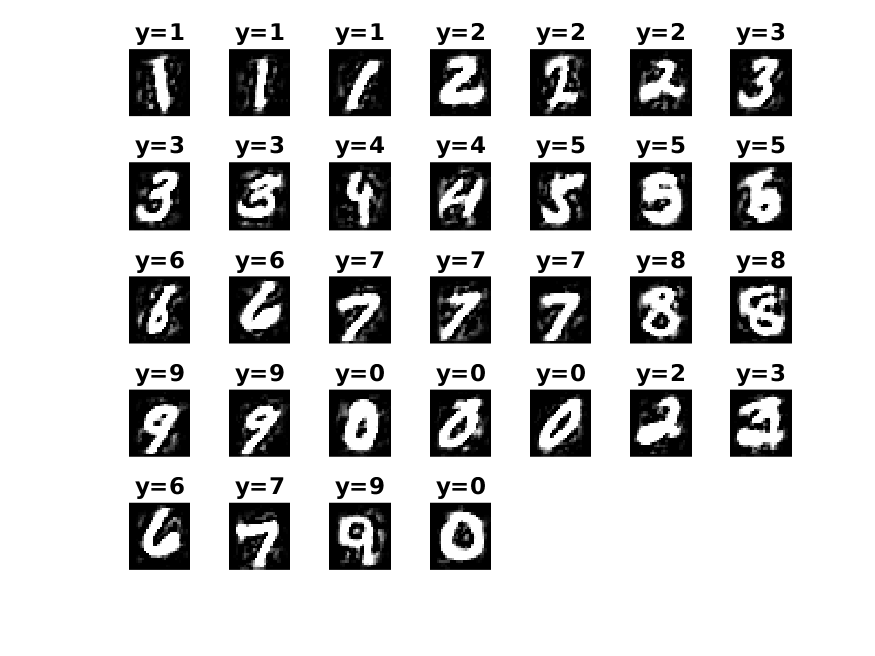
\includegraphics[width=0.65\columnwidth]{RunResults2/12.png}
\label{12}

\end{multicols}
\end{figure}
\newpage
\subsection{Fig 13}
\begin{figure}[h!]
\begin{center}
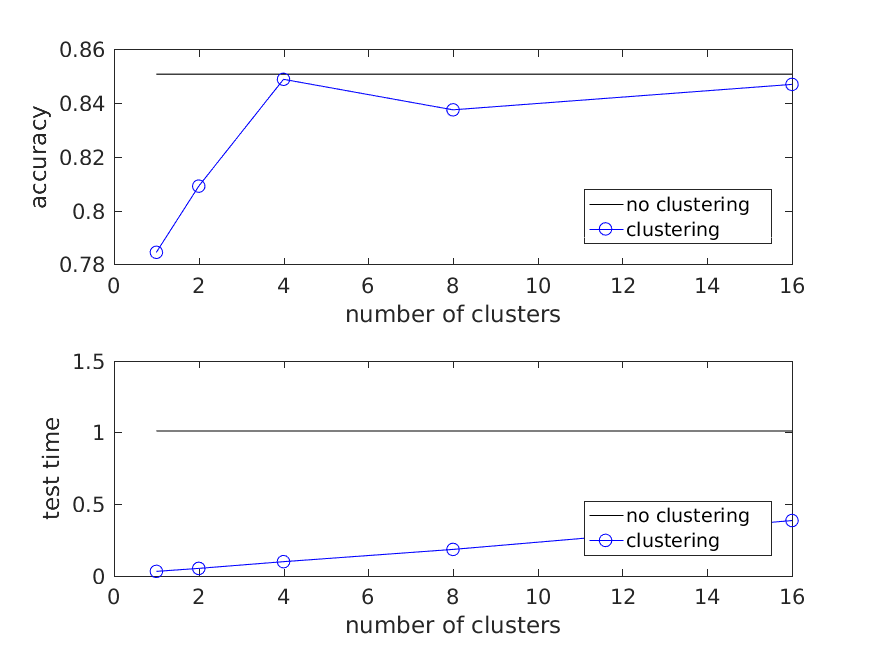
\includegraphics[width=0.5\columnwidth]{RunResults2/13.png}
\label{13}
\end{center}
\end{figure}

\subsection{Fig 14}
\begin{figure}[h!]
\begin{center}
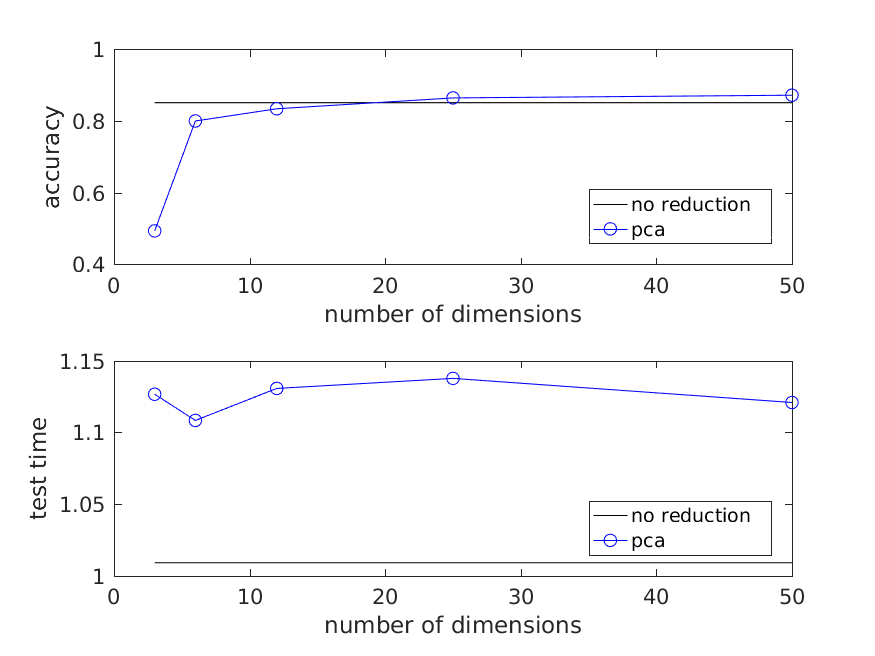
\includegraphics[width=0.5\columnwidth]{RunResults2/14.png}
\label{14}
\end{center}
\end{figure}

\section{Problem 3}
As discussed in class, $y_n \in {0,1,2, ... K-1}$ and label probabilities are defined as:
$$p(y_n=k|x_n,W) = \frac{exp(w_k^\top x_n)}{\sum_{l=1}^{K}exp(w_l^\top x_N)} = \mu_{nk}$$
\\
Log Likelihood is given as:
\begin{equation*}
\begin{aligned}
log(\prod_{n=1}^N p(y_n|x_n,W)) &=  \sum_{n=1}^N log(\mu_{ny_n}) \\
&=  \sum_{n=1}^N log(\frac{exp(w_{y_n}^\top)x_n}{\sum_{l=1}^K exp(w_l^\top x_N)}) \\ 
&= \sum_{n=1}^N [w_{y_n}^\top x_n - log(\sum_{l=1}^K exp(w_l^\top x_N))] \\ 
\end{aligned}
\end{equation*}
\newpage

Thus, Negative Log Likelihood is given by:
$$NLL(W) =  -\sum_{n=1}^N [w_{y_n}^\top x_n - log(\sum_{l=1}^K exp(w_l^\top x_N))]  $$

Now, taking it's derivative w.r.t 


\section{Problem 4}
\end{document}


